\documentclass{article}
\usepackage{amsmath, amssymb}
\usepackage[margin=1in]{geometry}
\usepackage{setspace}
\usepackage{graphicx}
\usepackage{multicol}
\usepackage[backend=bibtex]{biblatex}

\addbibresource{mbib.bib}

\doublespacing

\title{The R\"{o}ssler System}
\author{Steven Rosendahl}
\date{}

\begin{document}
\maketitle

In 1976, Otto R\"{o}ssler proposed a system of nonlinear ordinary differential equations that illustrated the simplest possible strange attractor. An attractor is a set of values towards which a system moves when initial conditions are \textit{near} the attractor; to call an attractor \textit{strange} means that the attractor exhibits fractal behavior. Often, strange attractors are associated with chaotic systems. R\"{o}ssler's strange attractor is a chaotic attractor that solves his proposed system
\begin{align}
	f(x,y,z) = \dot{x} & = -y-z     \\
	g(x,y,z) = \dot{y} & = x+ay     \\
	h(x,y,z) = \dot{z} & = b+z(x-c)
\end{align}
where $a,b,$ and $c$ are arbitrary values. R\"{o}ssler studied the effects that small (i.e. less than 1) $a$ and $b$ paired with a relatively large $c$ had on the system's chaotic behavior. One such plot is shown in figure \ref{fig:3dsys_01}.

We first want to analyze the stability of the critical points of the system. The Jacobian for this system can be found by constructing a matrix of partial derivatives for $f,g,$ and $h$.
\[
	J(x,y,z)=
	\left[
	\begin{array}{c c c}
		\frac{\partial f}{\partial x} & \frac{\partial f}{\partial y} & \frac{\partial f}{\partial z} \\
		\frac{\partial g}{\partial x} & \frac{\partial g}{\partial y} & \frac{\partial g}{\partial z} \\
		\frac{\partial h}{\partial x} & \frac{\partial h}{\partial y} & \frac{\partial h}{\partial z} \\
	\end{array}
	\right]
	=
	\left[
	\begin{array}{c c c}
		0 & -1 & -1  \\
		1 & a  & 0   \\
		z & 0  & x-c
	\end{array}
	\right].
\]
We now need to find the critical points of the system. We can accomplish this by solving $f=0,g=0,$ and $h=0$. Through the use of Mathematica's \texttt{Solve} command, we get
\begin{center}
	\texttt{Solve[f[x, y, z] == 0 \&\& g[x, y, z] == 0 \&\& h[x, y, z] == 0, \{x, y, z\}]}
\end{center}
\begin{gather}
	\left[
	x=\frac{1}{2}\left(c-\sqrt{c^{2}-4ab}\right),
	y=\frac{1}{2}\left(\frac{\sqrt{c^{2}-4ab}}{a}-\frac{c}{a}\right),
	z=\frac{c-\sqrt{c^{2}-4ab}}{2a}
	\right]\label{eq:csln1}\\
	\left[
	x=\frac{1}{2}\left(c+\sqrt{c^{2}-4ab}\right),
	y=\frac{1}{2}\left(-\frac{\sqrt{c^{2}-4ab}}{a}-\frac{c}{a}\right),
	z=\frac{c+\sqrt{c^{2}-4ab}}{2a}
	\right]\label{eq:csln2}.
\end{gather}

R\"{o}ssler's analysis focused on the behavior of the system for small $a$ and $b$. For simplicity, we can consider the solutions to (\ref{eq:csln1}) and (\ref{eq:csln2}) for very small $a$ and $b$. We now have
\begin{gather}
	\left[
	x=0,
	y=0,
	z=0
	\right]\label{eq:csln1sm}\\
	\left[
	x=c,
	y=-\frac{c}{a},
	z=\frac{c}{a}
	\right]\label{eq:csln2sm}.
\end{gather}
To find the behavior around the critical points given by (\ref{eq:csln1sm}), we evaluate the Jacobian at the appropriate points and find the eigenvalues of the system.
\[
	|J(0,0,0)-\lambda I| =
	\left|
	\left[
	\begin{array}{c c c}
		-\lambda & -1       & -1         \\
		1        & -\lambda & 0          \\
		0        & 0        & -c-\lambda
	\end{array}
	\right]
	\right| =
	(c-\lambda)(\lambda + 1)^{2}=0.
\]
Hence, the system has three eigenvalues: $\lambda=-i, \lambda=-i,$ and $\lambda = -c$ (we will assume here that $c > 1$). This implies that the system has an unstable focus node at the origin \cite{equilibria}. Figure \ref{fig:plot_cuts} shows various cuts of the system for various $z$ values; the system spirals in the $x-y$ plane, while moving towards and then away from the origin as $z$ moves from $-\infty$ to $\infty$. We can solve this linearized system by looking at the equation
\[
	\mathbf{\dot{x}} =
	\left[
	\begin{array}{c c c}
		0 & -1 & -1 \\
		1 & 0  & 0  \\
		0 & 0  & -c
	\end{array}
	\right]
	\mathbf{x}.
\]
Since we've already found the eigenvalues of the system, we can find the eigenvectors immediately.

\begin{minipage}{0.3\textwidth}
	\begin{gather*}
		\text{\underline{$\lambda=-i$}}\\
		\mathbf{\lambda_{1}}=\left[
		\begin{array}{c}
			-i \\
			1  \\
			0
		\end{array}
		\right].
	\end{gather*}
\end{minipage}
\begin{minipage}{0.3\textwidth}
	\begin{gather*}
		\text{\underline{$\lambda=i$}}\\
		\mathbf{\lambda_{2}}=\left[
		\begin{array}{c}
			i \\
			1 \\
			0
		\end{array}
		\right].
	\end{gather*}
\end{minipage}
\begin{minipage}{0.3\textwidth}
	\begin{gather*}
		\text{\underline{$\lambda=-c$}}\\
		\mathbf{\lambda_{3}}=\left[
		\begin{array}{c}
			\frac{c}{1+c^{2}}  \\
			-\frac{1}{1+c^{2}} \\
			1
		\end{array}
		\right].
	\end{gather*}
\end{minipage}

\noindent\\
\noindent Letting $\mathbf{\gamma}$ stand in for our constants, we get
\[
	\mathbf{x}(t) =
	\gamma_{1}e^{-it}\left[
	\begin{array}{c}
		-i \\
		1  \\
		0
	\end{array}
	\right] +
	\gamma_{2}e^{it}
	\left[
	\begin{array}{c}
		i \\
		1 \\
		0
	\end{array}
	\right] +
	\gamma_{3}e^{-ct}\left[
	\begin{array}{c}
		\frac{c}{1+c^{2}}  \\
		-\frac{1}{1+c^{2}} \\
		1
	\end{array}
	\right].
\]
Note that we choose to leave the $e^{it}$ in this form, since \textbf{${\lambda_{1}}$} and $\mathbf{\lambda_{2}}$ are linearly independent of each other. Figure \ref{fig:zero_sln} shows the behavior of this linearized system with two different sets of initial conditions. If we compare this to figure \ref{fig:3dsys_02}, we see similar behavior in the area of the graph with large $z$ values.

This represents only one of the equilibrium points of the system, however. We now need to analyze the linearized system near (\ref{eq:csln2sm}). In this case, we cannot let $a$ tend towards zero as we did in (\ref{eq:csln1sm}) since our roots rely on division by $a$.
\[
	\left|J\left(c,-\frac{c}{a},\frac{c}{a}\right) -\lambda I\right| =
	\left|
	\left[
	\begin{array}{c c c}
		-\lambda    & -1          & -1       \\
		1           & a - \lambda & 0        \\
		\frac{c}{a} & 0           & -\lambda
	\end{array}
	\right]
	\right| =
	\frac{ ac - a\lambda - c\lambda + a^{2}\lambda^{2} -a\lambda^{3}}{a}.
\]
Setting the determinant to $0$ and solving in Mathematica yields three distinct (and incredibly verbose) eigenvalues with $\lambda_{1}\in\mathbb{R}$ the other two complex conjugates of each other. Such behavior lends itself towards what is known as a \textit{saddle focus}, which is always unstable \cite{equilibria}. Figure \ref{fig:3dsys_02} displays the behavior of both equilibrium points. The spiral behavior can be seen in the $x-y$ plane, and the saddle behavior can be seen predominantly in the $z-x$ plane.

Again, we can solve the linearized system and analyze the behavior as we did with the system centered around $(0,0,0)$. Due to the complexity of the eigenvalues of this system, we let Mathematica determine the behavior. The command
\begin{center}
	\texttt{Eigenvectors[jcbn[x, y, z] /. \{x -> c, y -> -(c/a), z -> (c/a)\}]}
\end{center}
yields an unfriendly expression involving the \texttt{Root} command; in this case we will want to give concrete values to $c$ and $a$. Figure \ref{fig:3dsys_02} involves the behavior of the system at $a=0.14$ and $c=8.8$, so we will examine the resulting eigenvalues at those points.
\begin{center}
	\texttt{Eigenvectors[jcbn[x, y, z] /. \{x -> c, y -> -(c/a), z -> (c/a)\}]/.\{a -> 0.14, c -> 8.8\}}
\end{center}
results in the following three eigenvectors:

\begin{minipage}{0.3\textwidth}
	\begin{gather*}
		% \text{\underline{$\lambda=-i$}}\\
		\mathbf{\lambda_{1}}=\left[
		\begin{array}{c}
			-0.0022 \\
			-1.0003 \\
			1.0000
		\end{array}
		\right]
	\end{gather*}
\end{minipage}
\begin{minipage}{0.3\textwidth}
	\begin{gather*}
		% \text{\underline{$\lambda=i$}}\\
		\mathbf{\lambda_{2}}=\left[
		\begin{array}{c}
			0.0000174 - 0.12713i \\
			0.0159 + 0.00028i    \\
			1
		\end{array}
		\right]
	\end{gather*}
\end{minipage}
\begin{minipage}{0.3\textwidth}
	\begin{gather*}
		% \text{\underline{$\lambda=-c$}}\\
		\mathbf{\lambda_{3}}=\left[
		\begin{array}{c}
			0.0000174 - 0.12713i \\
			0.0159 + 0.00028i    \\
			1
		\end{array}
		\right].
	\end{gather*}
\end{minipage}

\noindent\\
\noindent We now have enough to for a general solution with $\mathbf{\gamma}$ in place of our constants.
\begin{gather*}
	\mathbf{x}(t) =
	\gamma_{1}e^{0.138t}\left[
	\begin{array}{c}
		-0.0022 \\
		-1.0003 \\
		1
	\end{array}
	\right] +
	\gamma_{2}e^{(0.00109-7.99i)t}\left[
	\begin{array}{c}
		0.0000174 - 0.12713i \\
		0.0159 + 0.00028i    \\
		1
	\end{array}
	\right] +\\
	\gamma_{3}e^{(0.00109+7.99i)t}\left[
	\begin{array}{c}
		0.0000174 + 0.12713i \\
		0.0159 - 0.00028i    \\
		1
	\end{array}
	\right].
\end{gather*}
Figure \ref{fig:nzero_sln} displays two parametric plots of the solution curves for different initial values. The curves exhibit a center-like behavior that looks like a spring. We can compare this to the actual curve seen in \ref{fig:3dsys_02}. This behavior is seen in the purple spiral in the $x-y$ plane of the graph.

We now know that both equilibrium points are unstable when we ignore $a$ and $b$ in comparison to $c$, but that behavior seems odd for an attractor. We analyzed the simple roots so that we would not have to try to symbolically analyze the eigenvalues of the system (see Figure \ref{fig:raw_ev} which gives one of the three eigenvalues of the linearized system when $a$ and $b$ are not ignored). We will now see the effects of the individual parameters on the system; to do this, we will have to hold two of the values constant. Throughout this discussion, we will consider $a=0.1, b=0.1$, and $c=8.8$ for the respective constant values.

Attractors are often associated with chaotic systems; as such, we will now examine various bifurcations on the R\"{o}ssler system. We have three variables that contribute to the chaos of the system: $a$, $b$, and $c$. R\"{o}ssler analyzed the system for relatively small $a$ and $b$, and we analyzed the stability of critical points when we neglected $a$ and $b$. The bifurcations will reveal behavior such as the periodicity and chaotic nature of the system. We will first analyze the effect that small changes to $a$ have on the system.

In order to analyze the effect of $a$ on the system, we need to hold $b$ and $c$ constant while changing $a$. The general strategy here will be to analyze the change on the eigenvalues of the linearized system, which will in turn allow us to . Figure \ref{fig:a_bifur_01} shows the effect that varying $a$ has on the system in the $x-y$ plane. As $a$ increases from $-\infty$, the system moves from a spiral sink to a center and finally to a saddle, moving from stable to semi-stable to unstable.

To see the change  in the eigenvalues, we can use the roots we found in (\ref{eq:csln1}) and (\ref{eq:csln2}). Replacing $a,b,$ and $c$ with our constant values yields the new Jacobians the we need to analyze.
\begin{equation}
	J_{\text{roots at (\ref{eq:csln1})}}=
	\left[
	\begin{array}{c c c}
		0                                  & -1 & -1                        \\
		1                                  & a  & 0                         \\
		\frac{8.8-\sqrt{77.44 - 0.4a}}{2a} & 0  & -4.4-0.5\sqrt{77.44-0.4a}
	\end{array}
	\right]\label{eq:a_mat_01}
\end{equation}
\noindent and
\begin{equation}
	J_{\text{roots at (\ref{eq:csln2})}} =
	\left[
	\begin{array}{c c c}
		0                                   & -1 & -1                          \\
		1                                   & a  & 0                           \\
		\frac{0.5(8.8\sqrt{77.44-0.4a})}{a} & 0  & 0.5(-8.8+\sqrt{77.44-0.4a})
	\end{array}
	\right]\label{eq:a_mat_02}
\end{equation}
\noindent yield different stability based on the small changes in $a$. For the Jacobian given in (\ref{eq:a_mat_01}), the eigenvalues change around $a=2$.
\begin{center}
	\begin{tabular}{l | l}
		$a=1.8$                      & $a=2.1$              \\
		\hline
		$\lambda_{1}=-8.77$          & $\lambda_{1}=-8.775$ \\
		$\lambda_{2}=0.899-0.435i$   & $\lambda_{2}=0.727$  \\
		$\lambda_{3}=0.899 + 0.435i$ & $\lambda_{3}=1.371$
	\end{tabular}
\end{center}
\noindent\\
\noindent We can clearly see that the stability changes from a stable focus node to an unstable saddle. As $a$ increases past $2.1$, the system continues to be unstable. In Figure \ref{fig:3dsys_02}, the purple section of the graph represents the portion of the system that we are analyzing. When $a>2$, the system is unstable at this point, causing trajectories to head away from the spiral and towards the orange section of the graph. We can also see what happens near the other fixed point. The eigenvalues of (\ref{eq:a_mat_02}) appear to change around $a=58.5$ and again around $a=193.6$.
\begin{center}
	\begin{tabular}{l | l | l}
		$a=58.5$                      & $a=58.6$             & $a=198.4$                   \\
		\hline
		$\lambda_{1}=58.483$          & $\lambda_{1}=-0.366$ & $\lambda_{1}=193.695$       \\
		$\lambda_{2}=-0.354 - 0.025i$ & $\lambda_{2}=-0.343$ & $\lambda_{2}=-4.39+0.1i $   \\
		$\lambda_{3}=-0.354 + 0.025i$ & $\lambda_{3}=58.58$  & $\lambda_{3}=-.0002-0.001i$
	\end{tabular}
\end{center}
\noindent\\
\noindent Here we see an unstable focus node changing into an unstable saddle. As $a$ increases, the system cycles between the a focus node and and unstable saddle, which is indicative of periodic behavior of the system.

We can now analyze the effect that changes in $b$ have on the system. For the fixed point in (\ref{eq:csln1}), we see a change in stability around $b=94.2$ and then again around $b=193.8$. At this fixed point, the eigenvalues change from a stable focus node to a stable node, and then into a set of three complex eigenvalues with non-zero real part. The final case is not a named type of equilibrium, and in fact it is not hyperbolic, so it does not tell us anything useful about the nonlinear system. It is unstable though, since at least one of the eigenvalues has a positive real part.
\begin{center}
	\begin{tabular}{l | l | l}
		$b=94.2$                           & $b=100$                 & $b=195$                           \\
		\hline
		$\lambda_{1}=-5.27985$             & $\lambda_{1}=-4.75948$  & $\lambda_{1}=-2.51539 - 6.51211i$ \\
		$\lambda_{2}=-1.08805 - 0.107786i$ & $\lambda_{2}=-1.93582$  & $\lambda_{2}=-1.78605 + 6.15461i$ \\
		$\lambda_{3}=-1.08805 + 0.107786i$ & $\lambda_{3}=-0.664116$ & $\lambda_{3}=0.00144 - 0.0167i$
	\end{tabular}
\end{center}
\noindent\\
\noindent Similarly, we can analyze the effect that perturbations in $b$ have on the fixed point given in (\ref{eq:csln2}). When varying $b$ from $0.1$ to 250, we do not see any change in the stability of the fixed point. It remains an unstable saddle focus, so we need not analyze this any further. It should be noted that we are considering fixed values for $a,b$, and $c$. If we chose other values and repeat this process, we may find that the changes to $b$ in this case actually do affect the system. We will not consider these cases, since the resulting work would take several more pages.

Finally, we can analyze the effect that $c$ has on the system. Similar to the effect of $b$ on (\ref{eq:csln2}), varying $c$ from $8.8$ to 2250 does not appear to change the stability of (\ref{eq:csln1}) and (\ref{eq:csln2}). In the first case, the fixed point remains an unstable saddle focus; in the latter case, the system also remains an unstable saddle focus. While $c$ may not change the stability of the fixed points, small changes in $c$ can yield both chaotic and periodic behavior. Figure \ref{fig:c_chaos} shows some of the values for which the attractor is periodic and chaotic. The figure considers the system with $a=b=0.1$, as we have done in our analysis. Notice that chaotic behavior creates infinite periods and that the system is subject to very small changes in $c$ (i.e. 12.6 to 13).

Overall, the R\"{o}ssler system is globally stable, but exhibits local instability based on initial conditions. This is a property of attractors; any trajectories that start outside of the attractor will eventually head towards the attractor. We can see this behavior in Figure \ref{fig:attractive}. The pink trajectory moves towards the attractor regardless of the local stability of the attractor itself (hence the name \textit{attractor}). This behavior allows us to conclude that the attractor will be globally stable.

The R\"{o}ssler system illustrates a simple attractor; as a result, it is not a useful system to model practical situations. Viewing the system as an illustration for more complex system provides insight to more complex examples. We have seen the effect that small changed in $a,b$, and $c$ have on the system, as well as the effect of initial conditions on solutions to the linear system. Luckily, the fixed points tend to remain hyperbolic as $a,b$, and $c$ change, which allows for easier analysis of the system. The R\"{o}ssler system provides an elegant view of a complex structure that would otherwise be very complicated.

\newpage
\clearpage
\section*{Plots and Graphics}
\begin{figure}[h]
	\centering
	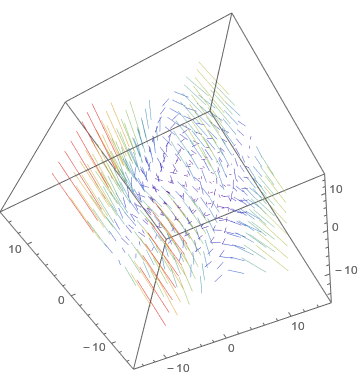
\includegraphics[scale=0.5]{vp_01.png}
	\caption{The R\"{o}ssler system with $a=0.2$, $b=0.1$, and $c=2.3$}
	\label{fig:3dsys_01}
\end{figure}

\begin{figure}[h]
	\centering
	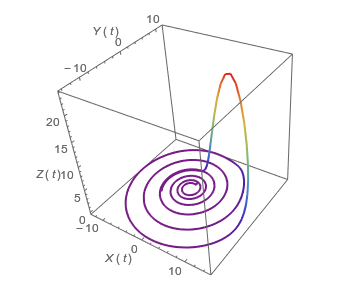
\includegraphics[scale=0.7]{attractor_a0p14_b0p2_c8p8}
	\caption{The R\"{o}ssler attractor with $a=0.14$, $b=0.2$, and $c=8.8$, courtesy of \cite{rossler_wf}}
	\label{fig:3dsys_02}
\end{figure}

\begin{figure}[h]
	\centering
	\begin{tabular}{c c}
		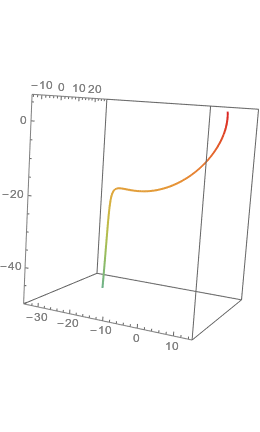
\includegraphics[scale=0.5]{gen_sln_01_01} & 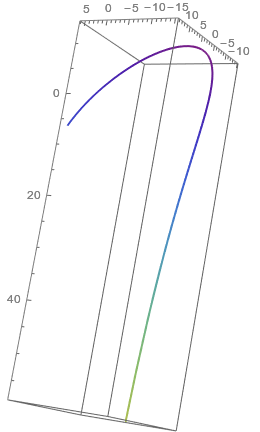
\includegraphics[scale=0.5]{gen_sln_01_02} \\
		$\gamma_{1}=-0.7$                          & $\gamma_{1}=-0.7$                          \\
		$\gamma_{2}=-0.7$                          & $\gamma_{2}=-0.7$                          \\
		$\gamma_{3}=-1$                            & $\gamma_{3}=1$                             \\
	\end{tabular}
	\caption{Two parametric plots for the linearized system around $(0,0,0)$ with different initial values}
	\label{fig:zero_sln}
\end{figure}

\begin{figure}[h]
	\centering
	\begin{tabular}{l r}
		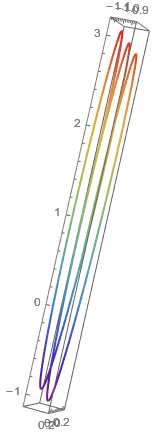
\includegraphics[scale=0.5]{gen_sln_02_01} & 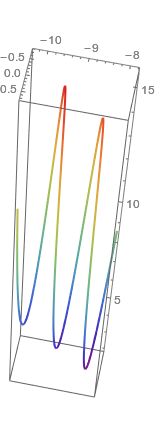
\includegraphics[scale=0.5]{gen_sln_02_02} \\
		$\gamma_{1}=1$                             & $\gamma_{1}=9$                             \\
		$\gamma_{2}=1$                             & $\gamma_{2}=-3$                            \\
		$\gamma_{3}=1$                             & $\gamma_{3}=-3$                            \\
	\end{tabular}
	\caption{Two parametric plots for the linearized system around $(c,-\frac{c}{a}, \frac{c}{a})$ with different initial values}
	\label{fig:nzero_sln}
\end{figure}

\begin{figure}[h]
	\centering
	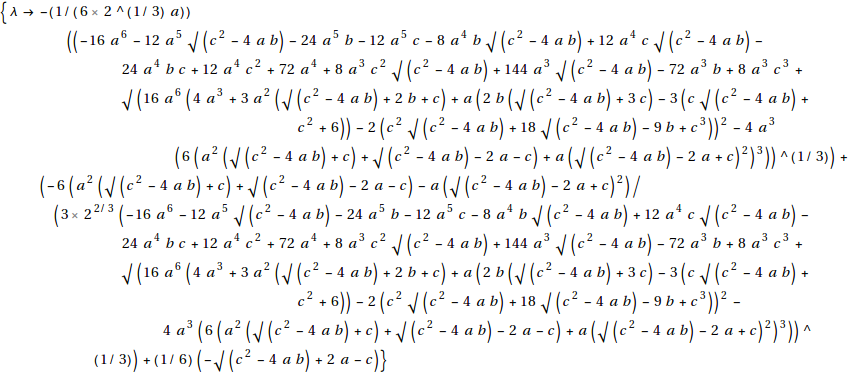
\includegraphics[scale=0.5]{messy_output}
	\begin{gather*}
		\{l\to -4.98425\}\\
		\{l\to 0.0961307\, -0.995341 i\}\\
		\{l\to 0.0961307\, +0.995341 i\}
	\end{gather*}
	\caption{Example of one raw eigenvalue and its corresponding evaluation at $a=0.2$, $b=0.2$, and $c=0.2$.}
	\label{fig:raw_ev}
\end{figure}

\begin{figure}[h]
	\centering
	\begin{tabular}{c c c}
		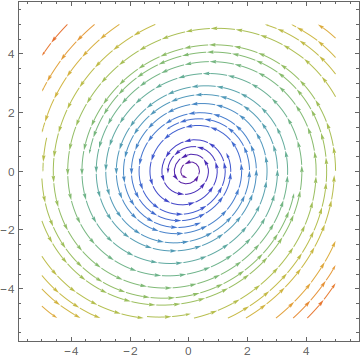
\includegraphics[scale=0.4]{a_bifur_n0p2} &
		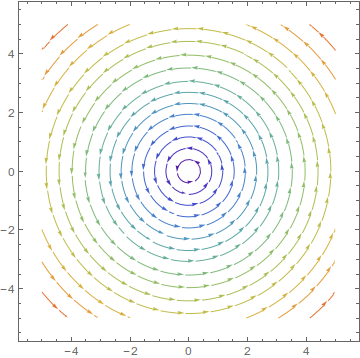
\includegraphics[scale=0.4]{a_bifur_n1p52656} &
		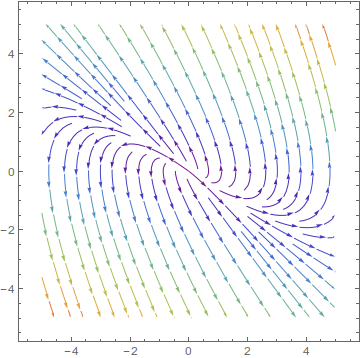
\includegraphics[scale=0.4]{a_bifur_2p1}\\
		$a=-0.2$ & $a=-1.52656$ & $a=2.1$
	\end{tabular}
	\caption{Three bifurcations for $a$ when $z=0$}
	\label{fig:a_bifur_01}
\end{figure}

\begin{figure}[h]
	\centering
	\begin{tabular}{c c}
		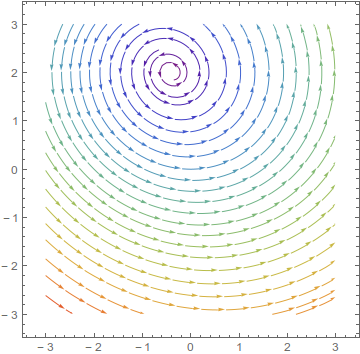
\includegraphics[scale=0.5]{spz-2} & 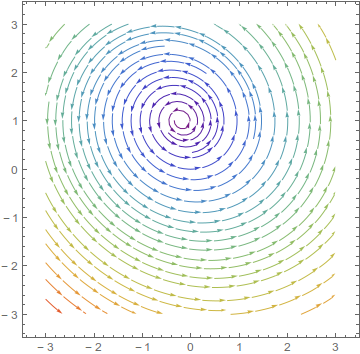
\includegraphics[scale=0.5]{spz-1} \\
		$z=-2$                             & $z=-1$                             \\
		\multicolumn{2}{c}{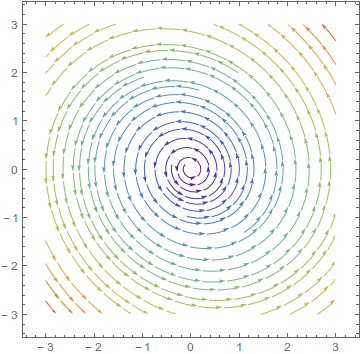
\includegraphics[scale=0.5]{spz0}}\\
		\multicolumn{2}{c}{$z=0$}\\
		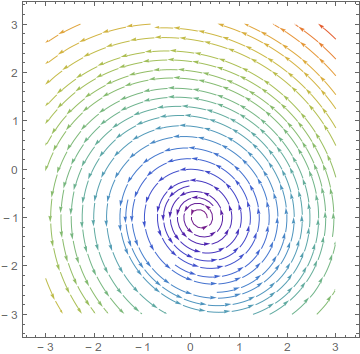
\includegraphics[scale=0.5]{spz1}  & 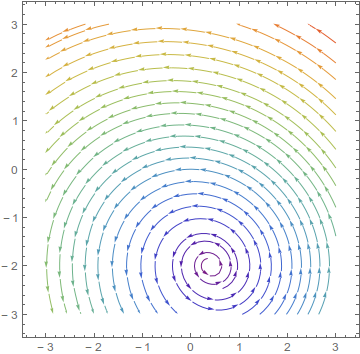
\includegraphics[scale=0.5]{spz2}  \\
		$z=1$                              & $z=2$
	\end{tabular}
	\caption{Several cuts of the stream plot given by Mathematica.}
	\label{fig:plot_cuts}
\end{figure}

\begin{figure}[h]
	\centering
	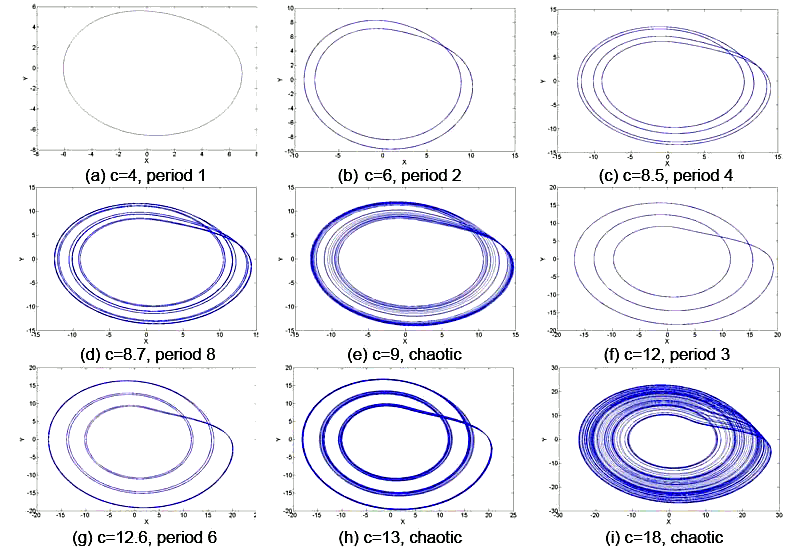
\includegraphics[scale=0.5]{varying_c}
	\caption{The chaotic behavior and periodicity of the system based on changed in $c$, courtesy of \cite{rossler_bifur}}
	\label{fig:c_chaos}
\end{figure}

\begin{figure}
	\centering
	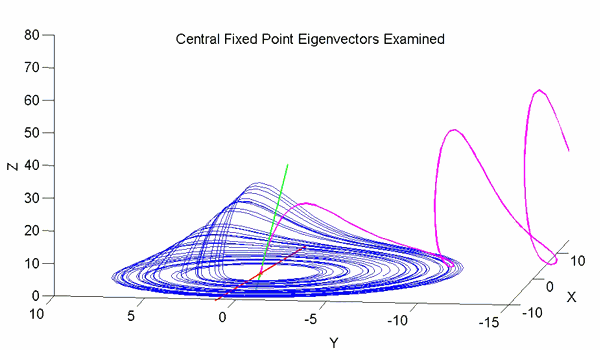
\includegraphics[scale=0.6]{attractive}
	\caption{An example of the global stability of the system. The pink trajectory heads towards the attractor and will remain there as $t\to\infty$ \cite{rossler_bifur} }
	\label{fig:attractive}
\end{figure}

\newpage
\clearpage
\nocite{*}
\printbibliography

\end{document}
